\documentclass[11pt,a4paper]{article}
\usepackage[hyperref]{acl2019}
\usepackage{times}
\usepackage{latexsym}
\usepackage{graphicx}

\usepackage{url}

\aclfinalcopy 

\newcommand\BibTeX{B\textsc{ib}\TeX}

\title{Assignment 2: E1-246 \\
Seq2Seq Model for Machine Translation}

\author{Aadesh Magare \\
  \texttt{aadeshmagare@iisc.ac.in} \\}

\date{}

\begin{document}
\maketitle
\begin{abstract}
  This is a report for assignment 2 of E1-246 course, Natural Language Understanding. The task was to implement a machine translation system for English to German and English to Hindi translations. The report contains experimental details and observations.
\end{abstract}

\section{Introduction}

A Seq2Seq model with attention was implemented for the translation task.
several attention mechanisms like scaled dot product, multiplicative, additive and key value attention were tried. The report contains details about the experiments and their comparison. further self attention for encoder and decoder was also explored and compared against.

\section{Datasets}
The English-German dataset was taken from WMT14 \cite{WMT}, which included Europarl v7, Common Crawl, News Commentary sources. It had over 4.5 M lines of text, out of which 1.5M were dropped for being exceedingly long length ( $>$20 words).
English-Hindi dataset was taken from \cite{ufal} which had total 0.25 M lines of text out of which around 9k were dropped ( $>$ 30 words). 
Developement and Test datasets were taken from WMT14. Corpus Bleu score is used as evaluation metric.

\section{Model}
The starter kit for project is taken from Stanford CS224n. \cite{cs224n} The Seq2Seq model has bidirectional LSTM encoder and a unidirectional LSTM decoder. The final model is trained with parameters in Table ~\ref{table1}.

In the interest of training time En-Hi model is trained for 5 epocs while En-De model is trained for 1 epoc, thus the Bleu score is less than what is expected but it should suffice for our comparison task.

\begin{table}[h]
\centering
\begin{tabular}{|l|l|}
\hline
\textbf{Parameter} & \textbf{Value} \\ \hline
Batch Size  & 32                          \\ \hline
Hidden Size  & 300                         \\ \hline
Embedding Dimensions & 300                         \\ \hline
\end{tabular}
\caption{Final Model Parameters}
\label{table1}
\end{table}

\section{Task 1: En-Hi Translation}

% ///////////////////////////////////////////////////////////////////

\subsection{Multiplicative Attention}
The model with multiplicative attention trained for 5 epocs achieves a Bleu score of 0.6138.
Training loss during the process initially drops rapidly to the level of 40 - 35 as seen in Figure ~\ref{fig1}. 

\begin{figure}[!htbp]
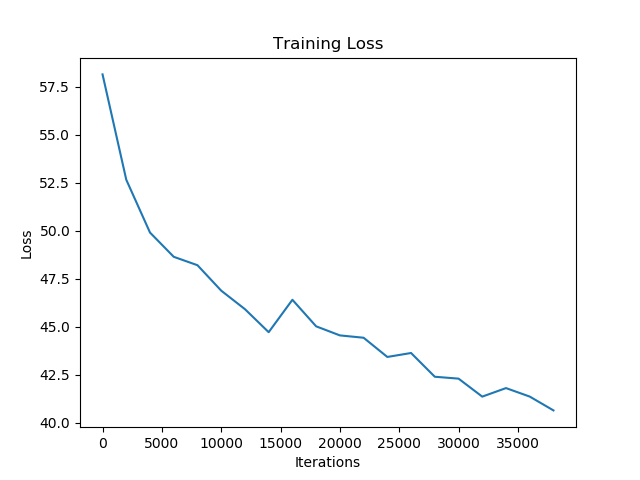
\includegraphics[width=\linewidth]{hi_mul_loss_1.png}
\caption{Initial Training Loss (Multiplicative)}
\label{fig1}
\end{figure}

The loss further keeps dropping at a slow rate. Similar behaviour is seen for Perplexity, it rapidly drops to the level of 500-450 as seen in Figure ~\ref{fig3} and further keeps dropping at slow rate.

% \begin{figure}[!htbp]
% 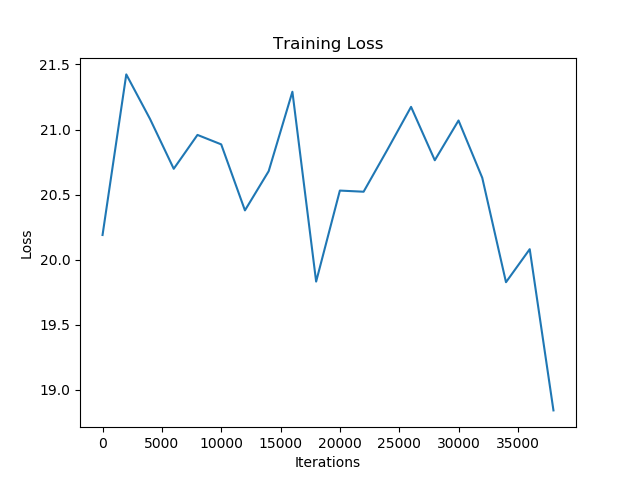
\includegraphics[width=\linewidth]{hi_mul_loss_2.png}
% \caption{Final Training Loss (Multiplicative)}
% \label{fig2}
% \end{figure}

\begin{figure}[!htbp]
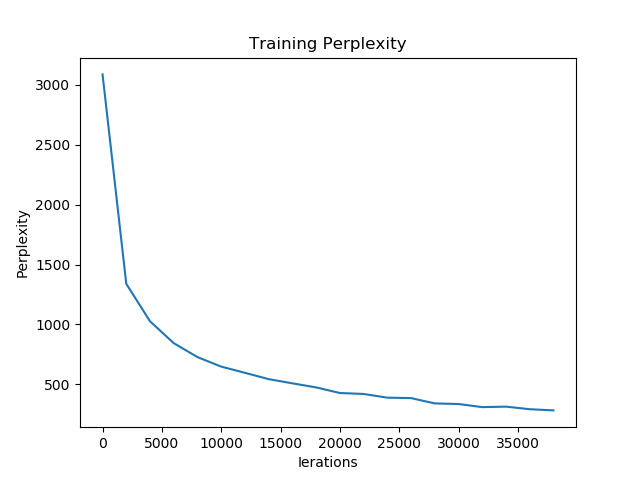
\includegraphics[width=\linewidth]{hi_mul_ppl_1.png}
\caption{Initial Perplexity (Multiplicative)}
\label{fig3}
\end{figure}

% \begin{figure}[!htbp]
% 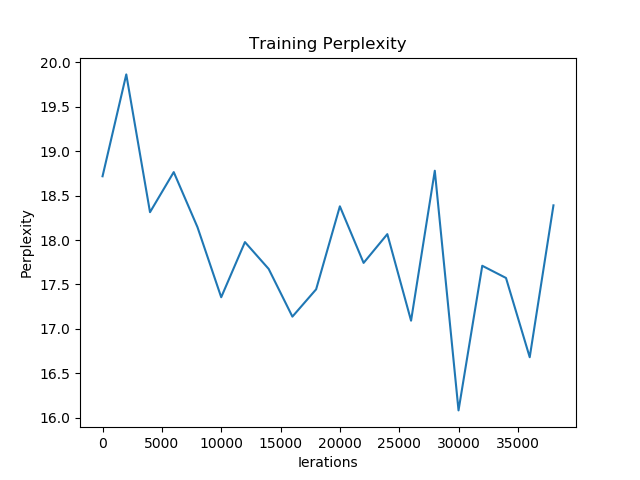
\includegraphics[width=\linewidth]{hi_mul_ppl_2.png}
% \caption{Final Perplexity (Multiplicative)}
% \label{fig4}
% \end{figure}
% //////////////////////////////////////////////////////////////////

\subsection{Scaled Dot Product Attention}
The model with scaled dot product attention trained for 5 epocs achieves a Bleu score of 2.1176.
Training loss during the process initially drops rapidly to the level of 40 - 30 as seen in Figure ~\ref{fig5}.

\begin{figure}[!htbp]
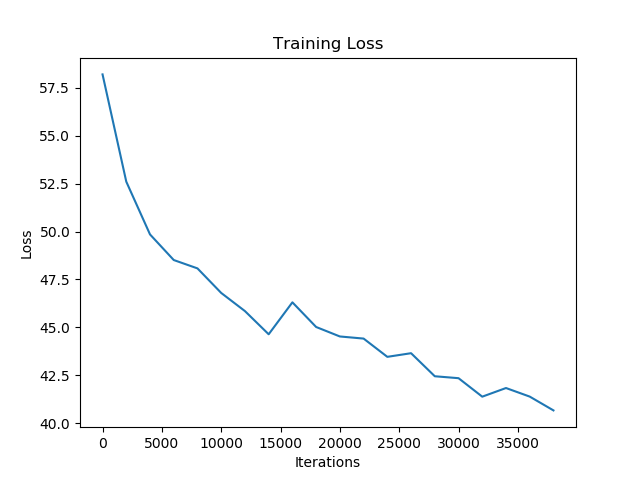
\includegraphics[width=\linewidth]{hi_dot_loss_1.png}
\caption{Initial Training Loss (Dot Product)}
\label{fig5}
\end{figure}

The loss further keeps dropping at a slow rate. Similar behaviour is seen for Perplexity, it rapidly drops to the level of 450-400 as seen in Figure ~\ref{fig7} and further keeps dropping at slow rate.


% \begin{figure}[!htbp]
% 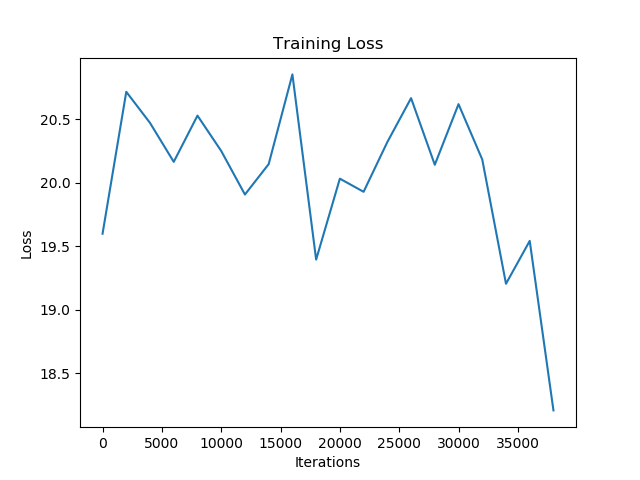
\includegraphics[width=\linewidth]{hi_dot_loss_2.png}
% \caption{Final Training Loss (Dot Product)}
% \label{fig6}
% \end{figure}

\begin{figure}[!htbp]
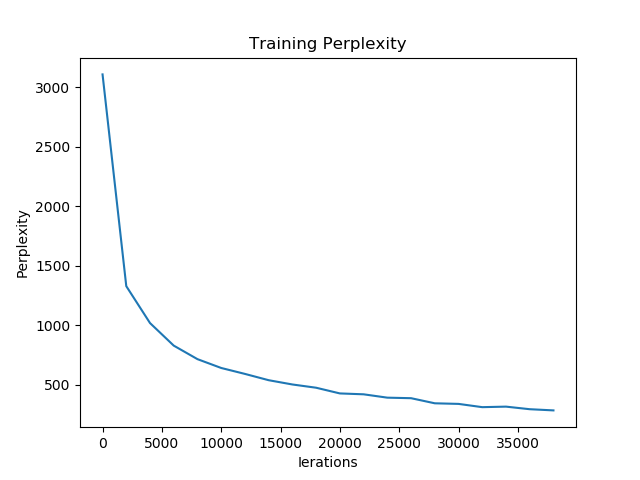
\includegraphics[width=\linewidth]{hi_dot_ppl_1.png}
\caption{Initial Perplexity (Dot Product)}
\label{fig7}
\end{figure}

% \begin{figure}[!htbp]
% 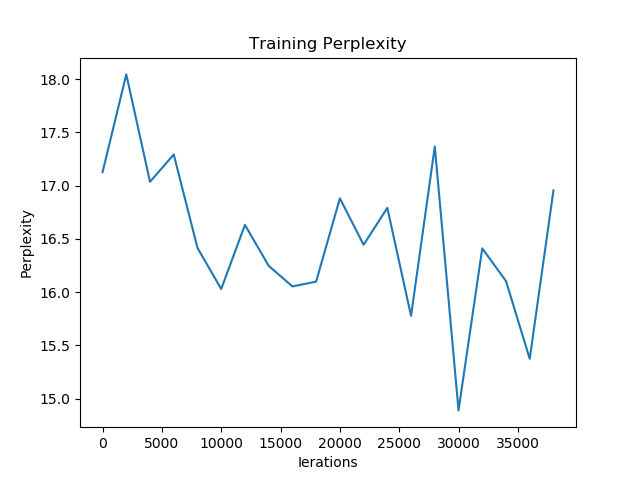
\includegraphics[width=\linewidth]{hi_dot_ppl_2.png}
% \caption{Final Perplexity (Dot Product)}
% \label{fig8}
% \end{figure}

% ////////////////////////////////////////////////////////////////////

\subsection{Additive Attention}

The model with additive attention trained for 5 epocs achieves a Bleu score of 0.8248.
Training loss during the process initially drops rapidly to the level of 55 - 50 as seen in Figure ~\ref{fig9}. 

\begin{figure}[!htbp]
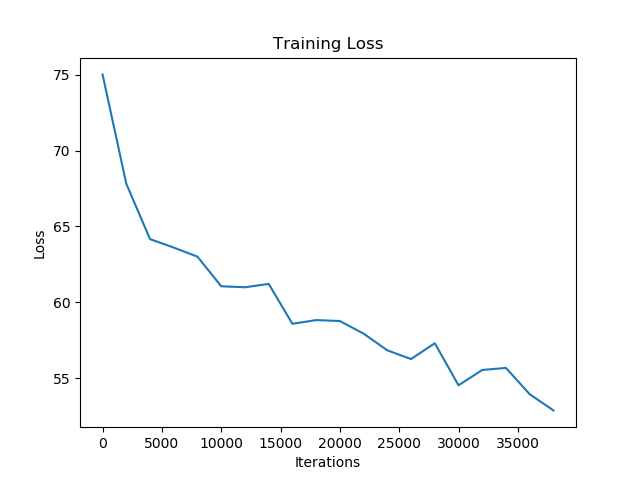
\includegraphics[width=\linewidth]{hi_add_loss_1.png}
\caption{Initial Training Loss (Additive)}
\label{fig9}
\end{figure}

The loss further keeps dropping at a slow rate. Similar behaviour is seen for Perplexity, it rapidly drops to the level of 250-200 as seen in Figure ~\ref{fig11} and further keeps dropping at slow rate.

% \begin{figure}[!htbp]
% 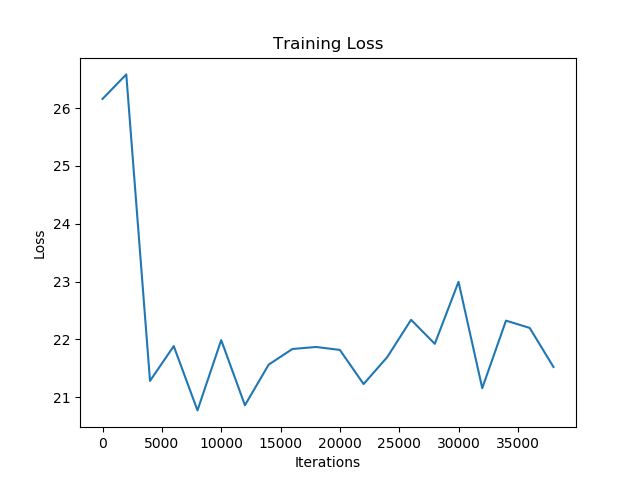
\includegraphics[width=\linewidth]{hi_add_loss_2.png}
% \caption{Final Training Loss (Additive)}
% \label{fig10}
% \end{figure}

\begin{figure}[!htbp]
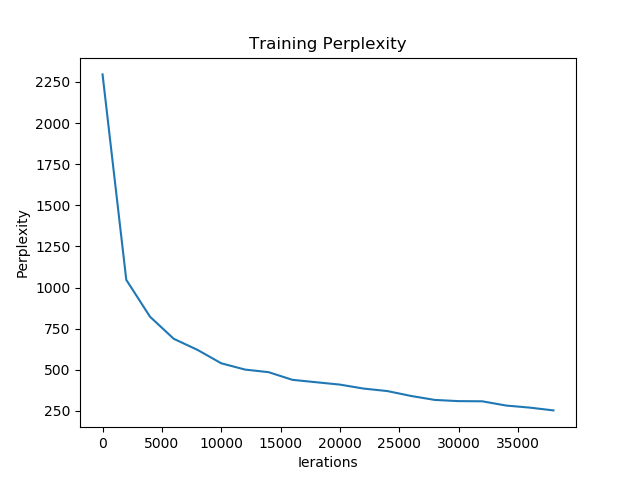
\includegraphics[width=\linewidth]{hi_add_ppl_1.png}
\caption{Initial Perplexity (Additive)}
\label{fig11}
\end{figure}

% \begin{figure}[!htbp]
% 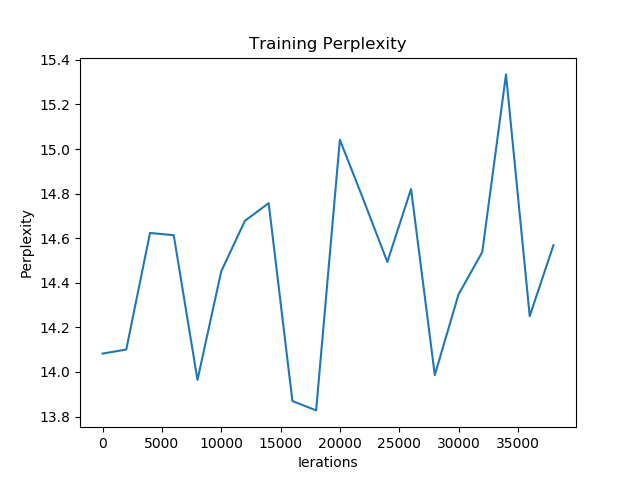
\includegraphics[width=\linewidth]{hi_add_ppl_2.png}
% \caption{Final Perplexity (Additive)}
% \label{fig12}
% \end{figure}

% ////////////////////////////////////////////////////////////////////

\subsection{Key Value Attention}

The model with key value attention trained for 5 epocs achieves a Bleu score of 0.6174.
Training loss during the process initially drops rapidly to the level of 50 - 40 as seen in Figure ~\ref{fig13}. 

\begin{figure}[!htbp]
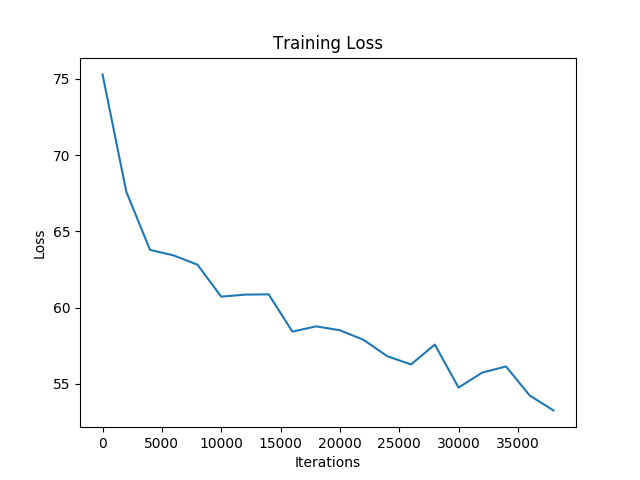
\includegraphics[width=\linewidth]{hi_key-value_loss_1.png}
\caption{Initial Training Loss (Key-Value)}
\label{fig13}
\end{figure}


The loss further keeps dropping at a slow rate. Similar behaviour is seen for Perplexity, it rapidly drops to the level of 400-300 as seen in Figure ~\ref{fig15} and further keeps dropping at slow rate.

% \begin{figure}[!htbp]
% 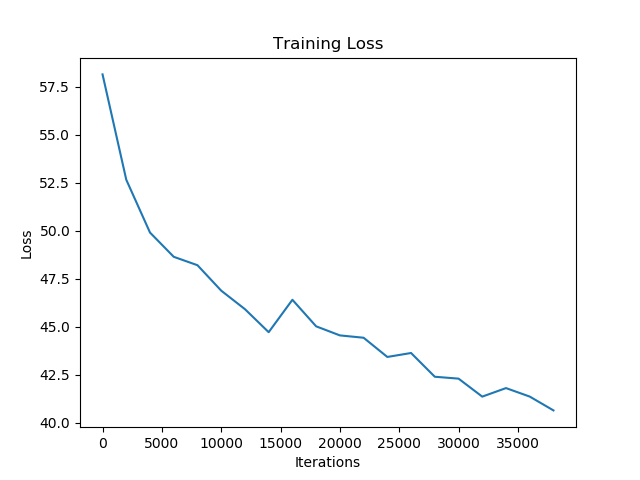
\includegraphics[width=\linewidth]{hi_mul_loss_1.png}
% \caption{Final Training Loss}
% \label{fig14}
% \end{figure}

\begin{figure}[!htbp]
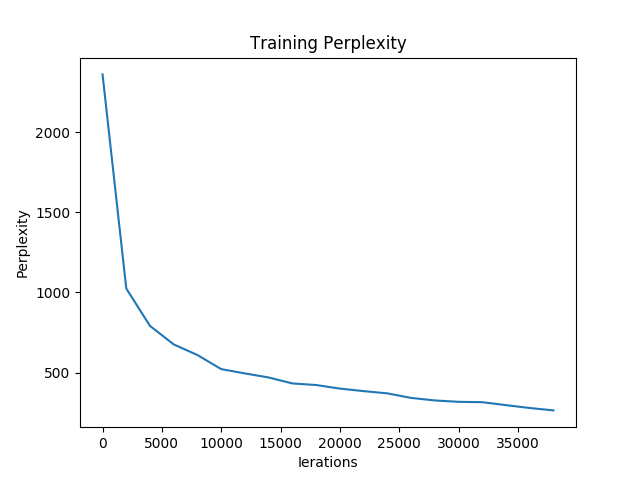
\includegraphics[width=\linewidth]{hi_key-value_ppl_1.png}
\caption{Initial Perplexity (Key-Value)}
\label{fig15}
\end{figure}

% \begin{figure}[!htbp]
% 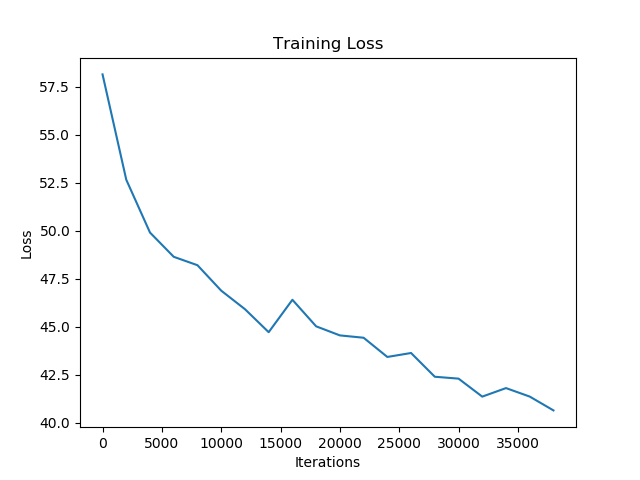
\includegraphics[width=\linewidth]{hi_mul_loss_1.png}
% \caption{Final Perplexity}
% \label{fig16}
% \end{figure}

% /////////////////////////////////////////////////////////////////////
% /////////////////////////////////////////////////////////////////////

\section{Task 2: En-De Translation}
% ///////////////////////////////////////////////////////////////////

\subsection{Multiplicative Attention}
The model with multiplicative attention trained for 1 epoc achieves a Bleu score of 0.1428.
Training loss during the process initially drops rapidly to the level of 50 - 45 as seen in Figure ~\ref{fig17}. 

\begin{figure}[!htbp]
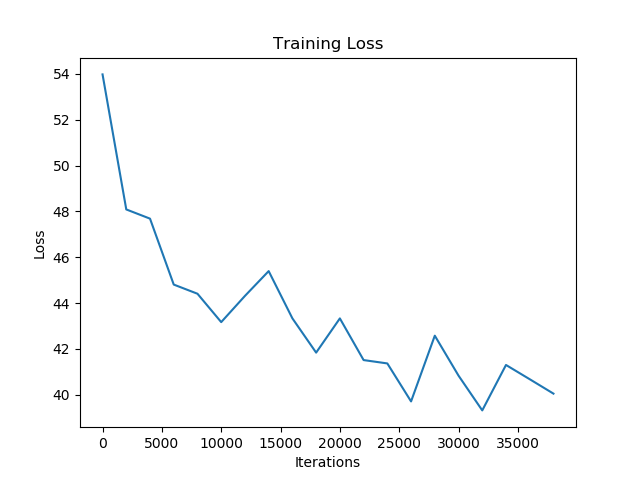
\includegraphics[width=\linewidth]{de_mul_loss_1.png}
\caption{Initial Training Loss (Multiplicative)}
\label{fig17}
\end{figure}

The loss further keeps dropping at a slow rate. Similar behaviour is seen for Perplexity, it rapidly drops to the level of 230-200 as seen in Figure ~\ref{fig19} and further keeps dropping at slow rate.

% \begin{figure}[!htbp]
% 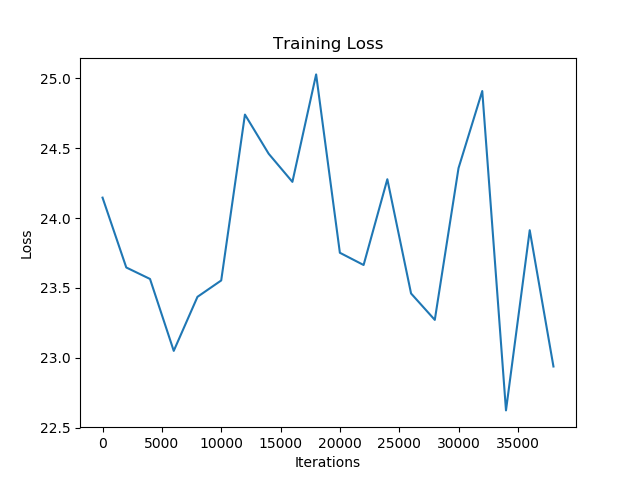
\includegraphics[width=\linewidth]{de_mul_loss_2.png}
% \caption{Final Training Loss (Multiplicative)}
% \label{fig18}
% \end{figure}

\begin{figure}[!htbp]
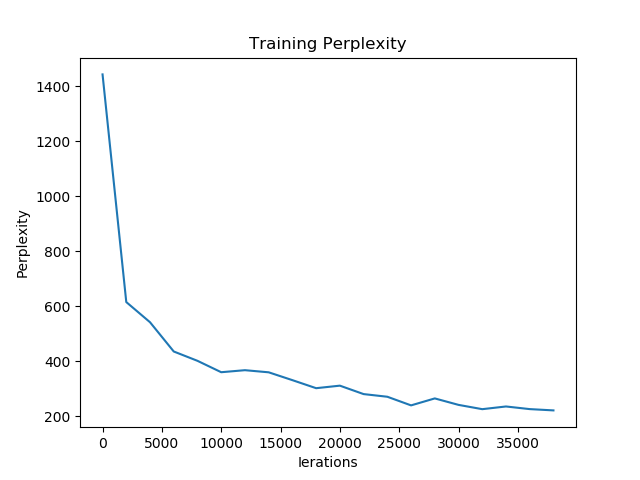
\includegraphics[width=\linewidth]{de_mul_ppl_1.png}
\caption{Initial Perplexity (Multiplicative)}
\label{fig19}
\end{figure}

% \begin{figure}[!htbp]
% 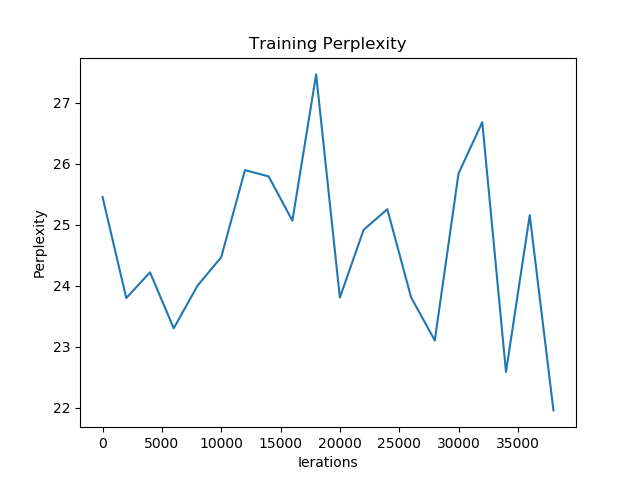
\includegraphics[width=\linewidth]{de_mul_ppl_2.png}
% \caption{Final Perplexity (Multiplicative)}
% \label{fig20}
% \end{figure}
% //////////////////////////////////////////////////////////////////

\subsection{Scaled Dot Product Attention}
The model with scaled dot product attention trained for 1 epoc achieves a Bleu score of 5.529.
Training loss during the process initially drops rapidly to the level of 40 - 35 as seen in Figure ~\ref{fig21}.
\begin{figure}[!htbp]
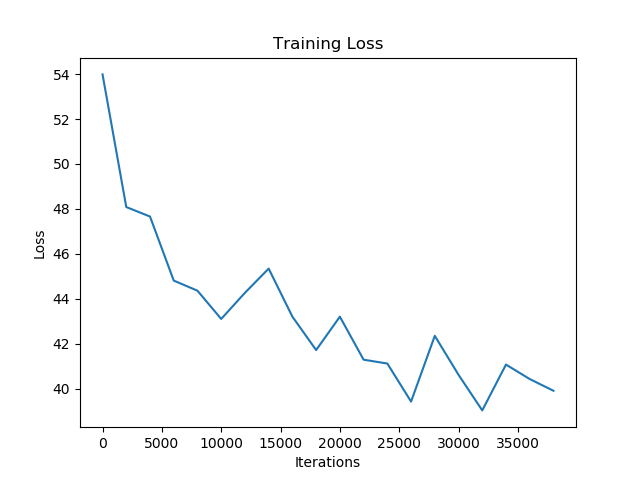
\includegraphics[width=\linewidth]{de_dot_loss_1.png}
\caption{Initial Training Loss (Dot Product)}
\label{fig21}
\end{figure}

The loss further keeps dropping at a slow rate. Similar behaviour is seen for Perplexity, it rapidly drops to the level of 220-200 as seen in Figure ~\ref{fig23} and further keeps dropping at slow rate.


% \begin{figure}[!htbp]
% 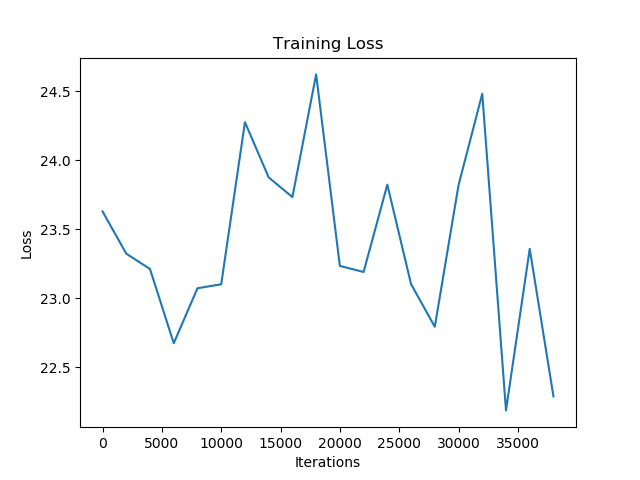
\includegraphics[width=\linewidth]{de_dot_loss_2.png}
% \caption{Final Training Loss (Dot Product)}
% \label{fig22}
% \end{figure}

\begin{figure}[!htbp]
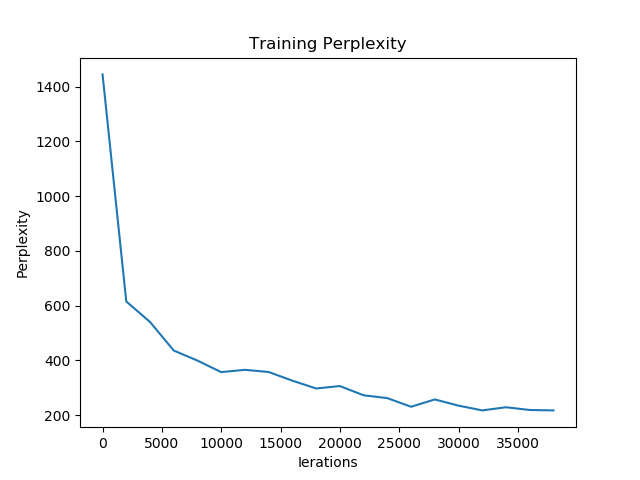
\includegraphics[width=\linewidth]{de_dot_ppl_1.png}
\caption{Initial Perplexity (Dot Product)}
\label{fig23}
\end{figure}

% \begin{figure}[!htbp]
% 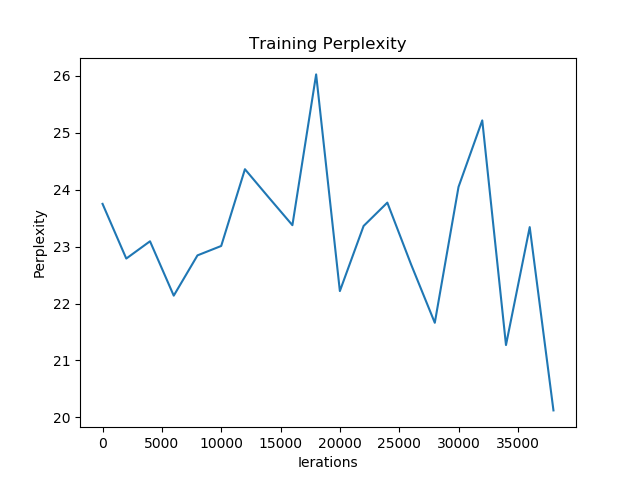
\includegraphics[width=\linewidth]{de_dot_ppl_2.png}
% \caption{Final Perplexity (Dot Product)}
% \label{fig24}
% \end{figure}

% ////////////////////////////////////////////////////////////////////
\pagebreak

\subsection{Additive Attention}

The model with additive attention trained for 1 epoc achieves a Bleu score of 0.2283.
Training loss during the process initially drops rapidly to the level of 45 - 40 as seen in Figure ~\ref{fig25}. 

\begin{figure}[!htbp]
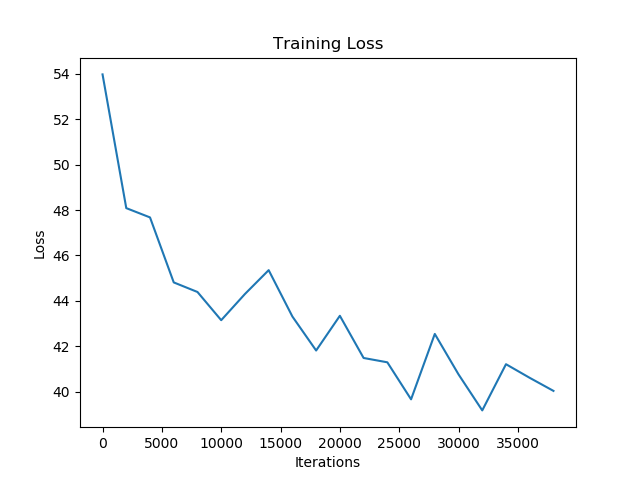
\includegraphics[width=\linewidth]{de_add_loss_1.png}
\caption{Initial Training Loss (Additive)}
\label{fig25}
\end{figure}

The loss further keeps dropping at a slow rate. Similar behaviour is seen for Perplexity, it rapidly drops to the level of 220-200 as seen in Figure ~\ref{fig27} and further keeps dropping at slow rate.

% \begin{figure}[!htbp]
% 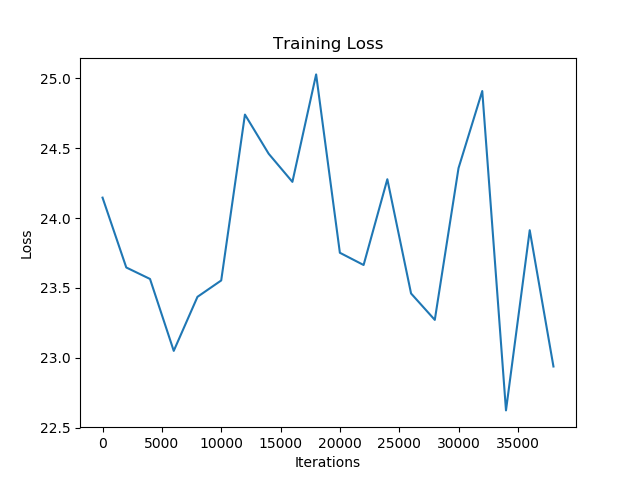
\includegraphics[width=\linewidth]{de_mul_loss_2.png}
% \caption{Final Training Loss}
% \label{fig26}
% \end{figure}

\begin{figure}[!htbp]
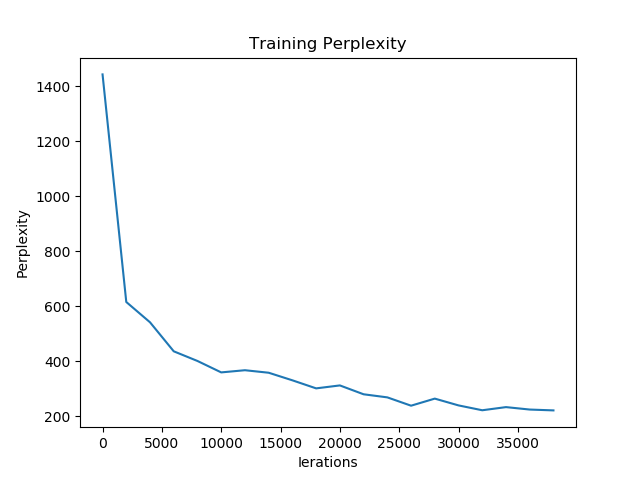
\includegraphics[width=\linewidth]{de_add_ppl_1.png}
\caption{Initial Perplexity}
\label{fig27}
\end{figure}

% \begin{figure}[!htbp]
% 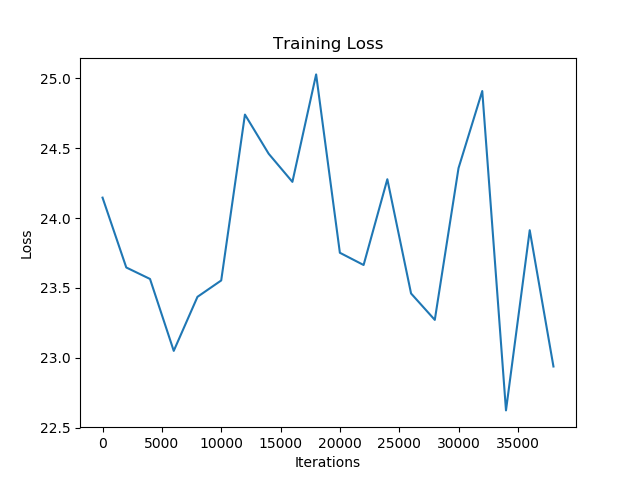
\includegraphics[width=\linewidth]{de_mul_loss_2.png}
% \caption{Final Perplexity}
% \label{fig28}
% \end{figure}

% ////////////////////////////////////////////////////////////////////
\pagebreak
\subsection{Key Value Attention}

The model with key value attention trained for 1 epoc achieves a Bleu score of 0.1294.
Training loss during the process initially drops rapidly to the level of 40 - 35 as seen in Figure ~\ref{fig29}. 

\begin{figure}[!htbp]
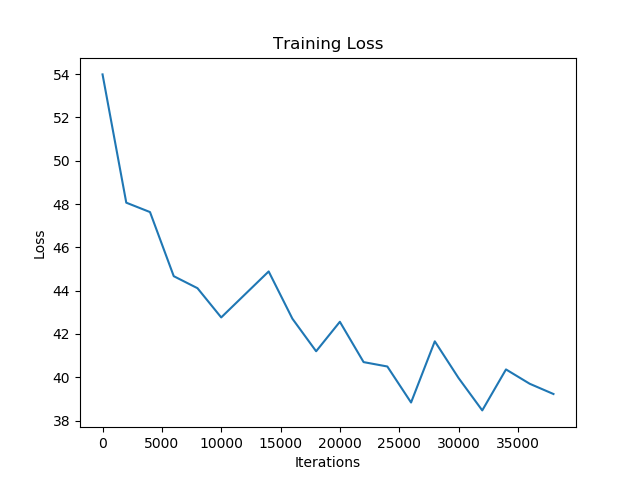
\includegraphics[width=\linewidth]{de_key-value_loss_1.png}
\caption{Initial Training Loss}
\label{fig29}
\end{figure}



The loss further keeps dropping at a slow rate. Similar behaviour is seen for Perplexity, it rapidly drops to the level of 220-200 as seen in Figure ~\ref{fig31} and further keeps dropping at slow rate.

% \begin{figure}[!htbp]
% 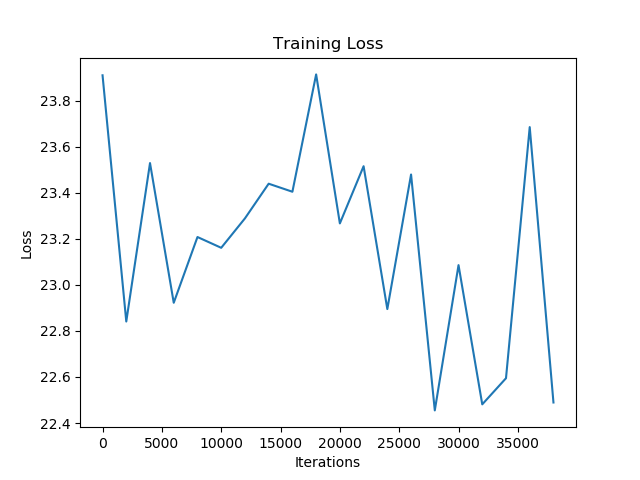
\includegraphics[width=\linewidth]{de_key-value_loss_2.png}
% \caption{Final Training Loss}
% \label{fig30}
% \end{figure}

\begin{figure}[!htbp]
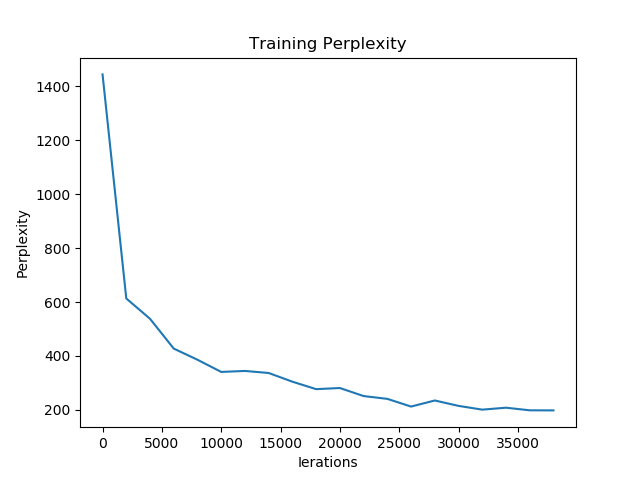
\includegraphics[width=\linewidth]{de_key-value_ppl_1.png}
\caption{Initial Perplexity}
\label{fig31}
\end{figure}

% \begin{figure}[!htbp]
% 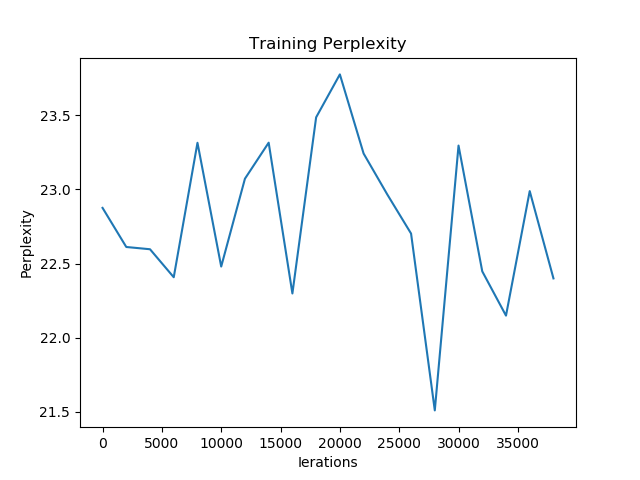
\includegraphics[width=\linewidth]{de_key-value_ppl_2.png}
% \caption{Final Perplexity}
% \label{fig32}
% \end{figure}

% //////////////////////////////////////////////////////////////////
% ///////////////////////////////////////////////////////////////////

\section{Self-Attention:}
Self-attention was implemented for encoder and decoder for the best performing model from previous sections. The training loss and perplexity follows similar expected behaviour as earlier where it initially drops rapidly and then slow down towards end of training. Self-attention however improves the Bleu score of model and shows a 1.2537 point improvement for En-Hi translation task and 0.13 point improvement for En-De task.

\section*{Repository:}
The project is available at \cite{GitHub} which contains code for experiment and additional plots.

\bibliography{acl2019}
\bibliographystyle{acl_natbib}

\end{document}
